%%%%%%%%%%%%%%%%%%%%%%%%%%%%%%%%%%%%%%%%%%%%%%%%%%%%%%%%%%%%%%%%%%%%%%%%%%%%%%%%
%2345678901234567890123456789012345678901234567890123456789012345678901234567890
%        1         2         3         4         5         6         7         8

\documentclass[letterpaper, 10 pt, conference]{ieeeconf}  % Comment this line out if you need a4paper

%\documentclass[a4paper, 10pt, conference]{ieeeconf}      % Use this line for a4 paper

\IEEEoverridecommandlockouts                              % This command is only needed if 
                                                          % you want to use the \thanks command

\newcommand{\ub}{\bar{u}}
\newcommand{\yb}{\bar{y}}
\newcommand{\wb}{\bar{w}}
\newcommand{\figref}[1]{Fig.~\ref{fig:#1}}
\overrideIEEEmargins       
\usepackage{todonotes}                              
\RequirePackage{graphicx}
\usepackage{subfigure}
\graphicspath{ {figures/} }
%\usepackage[tight,footnotesize]{subfigure}
\usepackage{fainekos-macros}

\newcommand{\hatodo}[1]{\todo{HA: #1}}
\newcommand{\hatodoin}[1]{\todo[inline]{HA: #1}}
\newcommand{\sAccu}{\epsilon}
\newcommand{\sDelay}{\delta}
\newcommand{\de}{(\sDelay,\sAccu)}

% See the \addtolength command later in the file to balance the column lengths
% on the last page of the document

% The following packages can be found on http:\\www.ctan.org
%\usepackage{graphics} % for pdf, bitmapped graphics files
%\usepackage{epsfig} % for postscript graphics files
%\usepackage{mathptmx} % assumes new font selection scheme installed
%\usepackage{times} % assumes new font selection scheme installed
\usepackage{amsmath} % assumes amsmath package installed
\usepackage{amssymb}  % assumes amsmath package installed

\title{\LARGE \bf
Anytime
}

\author{Authors% <-this % stops a space
\thanks{*This work was partially supported by the grants ???}% <-this % stops a space
\thanks{The Department of Electrical and Systems Engineering, University of Pennsylvania, Philadelphia, U.S.A.
        {\tt\small \{emails\}@seas.upenn.edu}}%
}


\begin{document}

\maketitle
\thispagestyle{empty}
\pagestyle{empty}

%\section{outline}

In autonomous cars, find numbers for power consumption of the perception chain.
(CMU, Shinpei)
\begin{enumerate}
	\item Introduction
	
	\item Motivating example: 
	\begin{itemize}
			\item hexrotor that is unstable/poor-performing with MPC because of actuation delay
			\item Operating at lowest delay (= worst performance) is not good either 
			\item How can we reduce the actuation delay while keeping a handle on estimation error? 			
	\end{itemize}
	Anytime control formulation explicity accounts for delay/error and optimizes over it.
	\\\quad A delay-error trade-off curve + control formulation that accounts for it
	
	\item Control problem and solution
	\begin{itemize}
		\item MPC control formulation 
		\item Solution
	\end{itemize}
	
	
	\item Delay-error curve 
	\begin{enumerate}
		\item Perception and estimation toolchain. Each component has knobs that make it anytime.
		\item Perception+estimation is a task with varying utility and execution time. The controller schedules the task with the best utility/execution time.
		\item this is also a utility/computation power trade-off.
		\item Example: corner detection for visual odometry
		\item Example: Yash's OpenCV toolchain: flowgraph and potentially curves.
	\end{enumerate}
	
	
	\item Experiment
	\begin{itemize}
			\item Show the curve on the quadrotor with ordroid (or maybe move to previous section)
			\item Computation power
			\item Experimental setup
			\item Take system from intro and show results with RAMPC: better performance/ stable.
			\item Degradation experiment: as we decrease control frequency and increase flying speed, performance degrades. How does degradation compare between the two.
			
	\end{itemize}

\end{enumerate}
\section{Introduction}
\label{sec:intro}

New:
nonlinear control with mpc on feedback linearized dynamics with state estimation error, input constraints, state constraints
	feedback linearization but no state constraints and identity T, no state uncertainty
	
state constraints
recursive feasibility with time-varying error sets

\textbf{Notation}.
Given two subsets $A,B$ of $\Re^n$, define their \textit{Minkowski sum} to be $A\oplus B \defeq \{a+b \such a\in A, b\in B\}$.
Define their Pontryagin difference to be $A\ominus B = \{c \in \Re^n \such c+b \in A \forall b \in B\}$


\section{Co-design of computation and control}

In the traditional design of the perception estimation and control algorithms in closed loop control systems, the controller is unaware of the implementation details of the perception module and the perception module is unaware of the requirements of the controller. In order to improve performance of over-loaded closed loop systems, we propose the co-design of both computation and control. The co-design involves modelling the perception tool-chain as a contract time algorithm which can choose its execution paths adaptively in order to realize a deadline given to it by the control algorithm. In addition, the controller is designed with the knowledge of the resulting operation modes of the perception algorithm, i.e. the performance versus computation time modes which the contract time perception algorithm can realize. This gives the controller the ability to leverage the flexible nature of the perception algorithm to maximize a performance measure while not being concerned about the internal workings of the perception algorithm. This allows a co-design of control and perception/estimation without violating the separability principle which is key to the design of closed loop control systems.

Figure \ref{} shows the closed loop architecture in a system with co-design of the perception and control algorithms. Unlike a closed loop system where the perception module is designed to operate at a fixed operating point, in the co-designed system, the controller can make the estimation algorithm switch to lower time/energy consuming modes based on the controller requirements. 


\section{Online Operation of Contract-Based Estimation and Control}
\label{controlProblem}
In this section we present the mathematical formulation of the online operation of the co-designed system presented in the previous section.
Specifically, we model the controller and physical system from Fig. ??, and demonstrate how the controller can, in real-time, use knowledge of the estimator's error-delay curve to decrease computation delay and power in an error-aware fashion.
This section is written in a tutorial fashion using a running example, with emphasis placed on the contract-based interaction between controller and estimator.

\section{Problem Formulation} \label{sec:formulation}

The control problem is as follows:

\begin{subequations}
\begin{align}
\text{Minimize } &l(x,u) \\
&\text{s.t.} \nonumber \\
\dot{x}&=f(x)+G(x)u \\
x&\in X\\
u&\in U
\end{align}
\end{subequations}

A discrete-time, periodic, state-estimator provides access to a state estimate with estimation error
\begin{subequations}
\begin{align}
\hat{x}(t)&=x(t)+e(t) \\ 
\text{where, } e(t) &\in E
\end{align}
\end{subequations}


\section{Contract based perception algorithms}
\label{delayErrorCurve}

In Section \ref{sec:codesign}, we postulated the existence of an Estimation Error vs Computation Delay ($\delta,\epsilon$) curve. % (the `error-delay curve').
This curve is used at every time step by the controller to determine the operating point $(\delta,\epsilon)$ for the next time step.
In this section we demonstrate in detail how such a curve may be obtained for particular applications and how points along the curve are realized at runtime by the contract based perception algorithms.

\subsection{Profiling and composing an anytime contract based perception algorithm}

Recall, in section \ref{sec:codesign} we briefly discuss how a contract based perception tool chain can be obtained by composing different version of the individual run-to-completion algorithms used in the perception algorithm. The first stage towards this is to identify the different individual components of the perception tool chain and identifying how to realize different computation time and accuracy versions of them. We refer to these different realizations  knobs for the perception algorithm, and the control knobs may be as simple as changing the number of iterations in a loop \cite{greenMS} or finding alternate implementations with different resultant execution times and performance for the same functionality. As a running example in this section to illustrate our methods, we consider a perception tool chain for object recognition from camera images. An overview of the flow and individual components of the tool chain is shown in figure \ref{}. 

This tool chain takes in a video stream and tracks an Object Of Interest (OOI) across the frames. The first stage of it is a pixel classifier that assigns to each pixel of the image (after potential pre-processing) the probability of its being a pixel of interest, i.e., of belonging to an OOI or being a part of the background. A binary image is then obtained which assigns the value 1 to pixels of interest, and 0 to all others. A knob here in the pixel classification stage is to realize different computation time and performance profiles, is the complexity of the probabilistic model used to detect whether a pixel belongs to the object of interest. The knob in this case is whether we choose a Gaussian Mixture Model (GMM) with fewer components, which would be faster but less accurate, versus a GMM with more components which will take more computation time but provide better classification performance. Knobs where we over fit the training data are removed by cross-validation stage as is standard. Next, filtering and a Connected Components (CC) algorithm is run on the binary image to get rid of noise in the classification process and segment its 1-valued pixels into disconnected objects. A shape classifier is then run on each object to determine whether it is an object of interest or not. 
% the pixel classifier is a Gaussian Mixture Model (GMMs), whose knob is the number of Gaussians in the mixture.
In our implementation for the object detector that we use as the illustrative example here, the pixel classifier is a GMM based classifers with the number of knobs being the number of components in the GMM as discussed above. The filtering and connected components algorithm are lumped into one stage and have a two-valued knob to choose between a 4-connected and 8-connected component implementation. The shape classifier is also a GMM, but the knob for it is the number of shape features resulting in Gaussians in different dimensions being fit, and hence resulting in different computation time and classification accuracy.
% The number of Gaussian components for the shape classifier is fixed since we know in advance the number of objects in the training and test sets.
In the given setting the number of knob settings for the entire chain is $K$ = (\#Gaussians for pixel classifier, \#neighbors for CC, \#features for shape classifier), and has a total of $3 \times 2 \times 2 = 12$ values.

Note that for any given algorithm in the chain, the relation between knob value and quality of output is not necessarily monotonic. The pixel and shape classifiers are machine learning algorithms that need to be trained on a training set before being used and like all machine learning algorithms, their output quality for a given knob setting will depend on the actual data set. For the object detection algorithm we use for illustration in this section, we use images from the \textbf{<what?>} dataset where each image is of size 1200x1600 pixels. The same is a fortiori true of the quality of the output of the entire chain. This is also reflected in figure \ref{}, where the solid line shows the mean perception error (measured as the 2-norm of the x,y co-ordinates of the centroid of the object and the estimated centroid from the object recognition algorithm) and the $90^{th}$ percentile execution time for the different knob settings.

The second stage to composing a contract based perception algorithm is to again use the training data to profile all the possible combinations of knobs through an extensive training and validation phase. This profiling gives us: a) Not only the output quality (or accuracy) of the perception tool chain under consideration, but also b) probability distributions for execution times for the stages of the perception tool chain under different knob settings. Note, since intermediate qualities are not easily measurable or assignable for some of the blocks of the tool chain (e.g. Connected Components) and for many other algorithms in general, we assign quality (or accuracy) distributions to the realizations of the complete tool chain by composing together different knob settings. Note, this profiling stage is done at offline at design time and provides us information that we use at runtime.

\subsection{Decision tree based run-time execution of the contract based perception algorithm}

After the contract based perception algorithm has been composed and the execution time distributions of its individual components and the quality distributions from composing together various knob settings have been profiled, we can represent the offline profiled algorithm as a decision tree as shown in figure \ref{} for run-time decisions. This decision tree based representation, where edges represent individual functions for different knobs, e.g. GMM based pixel classifier with 3 components, edges have assigned to them the execution time distributions of the functions they represent. Also, paths from the top of the tree to a leaf represent one particular realization of the tool chain and have assigned to them distributions for accuracy of the algorithm. The decision of selecting which knob setting to use for a particular stage for a given criteria can now be posed as an optimization problem for edge selection in the decision tree. For example, consider the case where we want to minimize the perception error while meeting a time deadline with a given high probability, the problem can be written as \textbf{<insert equation here>}. This problem can be re-solved after each stage is executed, allowing the algorithm the flexibility to re-optimize its execution path (or knob settings) after obtaining updated information on time consumed in the past stages.

This decision tree based approach is the equivalent of selecting different versions of tasks (knobs for stages) and scheduling them in sequential order to best perform the object recognition task while maximizing utilization (or estimation accuracy) and meeting the given time contract or deadline with a high probability. Figure \ref{} shows the different task versions for each stage and the resulting schedule based on the knob settings for the stages.




Specifically, we consider two different visual perception tool chains, where each tool of the chain has a knob that tunes its performance.
These knobs can be used to profile the tool chain and obtain its error-delay curve on particular platforms.
Because power consumption is correlated to computation time, the error-delay curve can also be viewed as an error-power curve.
The power consumption of the estimator task can be included in the control cost function using the $\alpha$ term of Eq.??.
Thus, the controller can save power by selecting operating modes $(\delta,\epsilon)$ that achieve the control objectives at a lower energy cost.



% subsection
\subsection{FAST corner detector for visual odometry}

The first perception algorithm we consider is the FAST corner detector~\cite{rosten_2006_machine} which we use for the visual odometry on a hex-rotor with a downward facing camera in the case study (see section \ref{sec:experiments} .
FAST detects corners in an image can be tracked across video frames to perform self-localization by a moving robot \cite{}. 
In real-time this closed loop control system that flies the hex-rotor, it is important to detect corners at frame rate or faster in order to provide a timely state estimate to the control algorithm.
The number $\#C$ and quality of corners detected in a frame directly affects the runtime of the corner detector and the resulting quality of the state estimate. Generally speaking, detecting more corners requires a longer runtime, and results in better self-localization as long as we are analysing a feature rich scene, i.e., \emph{assuming acceptable quality of the detected corners}. Thus the number $\#C$ of corners is a knob which can be varied to obtain an error-delay curve for self-localization with FAST corner detection based visual odometry. 
If the scene is not rich enough in features, and a sizeable fraction of the $\#C$ corners are of poor quality (i.e., unstable or hard to track across frames), then we can expect the self-localization error to actually increase as the poor quality, unstable corners detected add noise to the odometry process. 


Fig.~\ref{fig:fast} shows the error-delay curve of self-localization error using the FAST corner detector~\cite{rosten_2006_machine}.
The curve was obtained on an Odroid U3 [??], which is a quadcore \hatodoin{complete odroid specs}.
For each value of the knob $\#C$ (i.e., each requested number of corners), we ran the corner detector on a video sequence shot by a downward facing camera on-board a hexarotor while flying certain pre-set patterns.
The corners and some auxiliary data are then fed to a self-localization algorithm.
Ground truth for computing the self-localization error was obtained from the Vicon system which \hatodoin{half-sentence on what vicon does.}
As we repeat each flight several times, this results in a distribution of $(\delta,\epsilon)$ values for each value of $\#C$. 
We retained the $90^{th}$ percentile values for $\delta$ and $\epsilon$, since these are used as worst-case estimates by the controller of Section \ref{controlProblem}.
It can be seen that a larger number of requested corners produces a smaller estimation error and longer runtime.
Starting at 250 corners, the error increases, however. 

We hypothesize this is due to the decreasing quality of the corners being returned by FAST.
\begin{figure}[t]
\centering
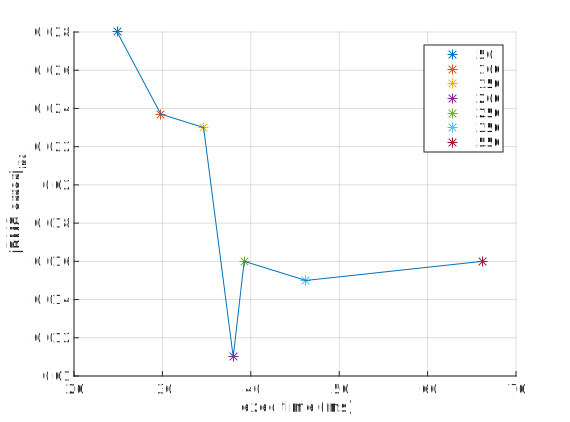
\includegraphics[width=0.7\linewidth]{figures/init_eps_delta_90th}
\caption{Error-delay curve for the FAST corner detector running on the Odroid U3}
\label{fig:fast}
\end{figure}

Fig.~\ref{fig:fastErrVsPower} shows the power consumption vs estimation error, which correlates well with Fig.~\ref{fig:fast}.
\begin{figure}[t]
	\centering
	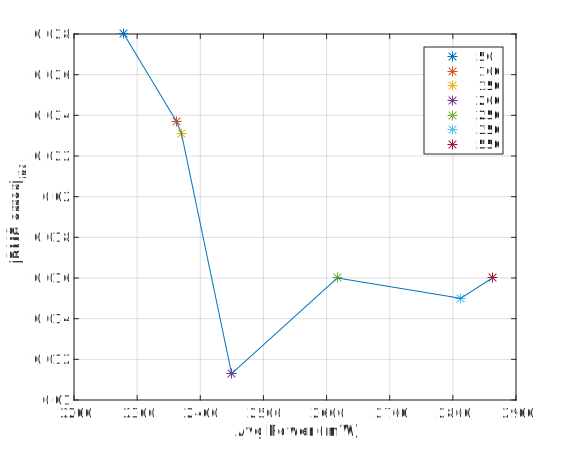
\includegraphics[width=0.7\linewidth]{figures/errVsPower}
	\caption{Error-delay curve for the FAST corner detector running on the Odroid U3}
	\label{fig:fastErrVsPower}
\end{figure}
% subsection
%

\subsection{A contract time object recognition tool chain}

Our second example is a more complete perception tool chain shown in Fig.~\ref{fig:chain}.
\begin{figure}[t]
	\centering
	\includegraphics[width=0.9\columnwidth]{figures/chain}
	\caption{Visual perception toolchain for object detection. The height of a block indicates output error, while width indicates runtime. The red path indicates one particular execution path which trades error for runtime at each stage.}
	\label{fig:chain}
\end{figure}
The tool chain takes in a video stream and tracks an Object Of Interest (OOI) across the frames.
The pixel classifier assigns to each pixel of the image (after potential pre-processing) the probability of its being a pixel of interest, i.e., of belonging to an OOI.
A binary image is then obtained which assigns the value 1 to pixels of interest, and 0 to all others.
A Connected Components (CC) algorithm is run on the binary image to segment its 1-valued pixels into disconnected objects.
A shape classifier is then run on each object to determine whether it is an object of interest or not.
The pixel and shape classifiers are machine learning algorithms that need to be trained on a training set before being used.
In our implementation of this chain, the specific algorithms and their knobs are as follows:
the pixel classifier is a Gaussian Mixture Model (GMMs), whose knob is the number of Gaussians in the mixture.
The connected components algorithm has a two-valued knob to choose between a 4-connected and 8-connected component implementation.
The shape classifier is also a GMM, but the knob for it is the number of shape features.
The number of Gaussian components for the shape classifier is fixed since we know in advance the number of objects in the training and test sets.
Thus the knob for the entire chain is $K$ = (\#Gaussians for pixel classifier, \#neighbors for CC, \#features for shape classifier), and has a total of $3 \times 2 \times 2 = 12$ values.
Note that for any given algorithm in the chain, the relation between knob value and quality of output is not necessarily monotonic.
Like all machine learning algorithms, it will depend on the actual data set.
The same is a fortiori true of the quality of the output of the entire chain.

Fig.~\ref{fig:chainErrorDelay} shows the \emph{perception error}-delay curve for the object detection chain.
The perception error is the difference between the estimated centroid of the OOI and the true centroid of the OOI.
If the chain fails at finding the object in the frame, we assign that frame a constant error drawn from the errors found on other frames.
Each point on the curve was obtained by training the tool chain with the associated knob value, and then running the trained tool chain on the test set to obtain the $(\delta,\epsilon)$ values.
The plotted error value is the average error over all images in the test set.
The fact that the error \emph{increases} in some points despite increasing computation time can be explained by the remark made earlier: namely that the effect of a knob value is not necessarily monotonic on quality.
Moreover, the effect of a change to one algorithm of the chain might outweigh changes to other algorithms.
This makes profiling the end-to-end tool chain all the more important.
Thus, online, the controller can ignore the modes that show a degraded performance despite a higher energy cost.

This curve can then be turned into an estimate error-delay curve by incorporating it into an estimation algorithm.
\begin{figure}[t]
	\centering
	\includegraphics[width=0.9\columnwidth]{figures/chainErrorDelay}
	\caption{Perception error vs Delay curve for the chain of Fig.~\ref{fig:chain}}
	\label{fig:chainErrorDelay}
\end{figure}
More generally, such curves can be obtained for a given state estimator by identifying the knobs that control the quality and runtime of the estimator, and profiling the estimator's code at the various values of the knobs.
In effect, this gives us several Estimator tasks, each with a different utility.
I.e., each such task strikes a different balance between computation time and quality of estimate.
At time step $k$, the controller schedules the task with the best trade-off for step $k+1$, in the sense of optimizing the cost function in Eq.??


\section{Case Study: Real-time feedback control of a hexrotor with contract based estimation and robust control}
\label{sec:experiments}

\subsection{Experimental setup}
To evaluate our methodology on a real platform, we applied it to a hexrotor with the Odroid-U3 as a computation platform, running the Robot Operating System (ROS) \cite{ROS288} in Ubuntu. For the evaluation, the hexrotor is tasked with repeatedly following a given circular trajectory.
As can be seen in Fig.~\ref{fig:time_ecdf}, the visual odometry algorithm can occcasionaly take a long time to give a pose estimate. In our formulation in section \ref{robustMPC} we have assumed that the estimator satisfies the $(\delta, \epsilon)$ contract requested by the controller. Thus, to ensure that the estimator fulfills the contract and that the mathematical guarantees provided by our RAMPC formulation hold, instead of using the visual odometry algorithm to fly the robot, 
we injected delays and errors into the measurements from Vicon, which is a high accuracy localization system. 
These delays and errors were selected from the $\Delta$ curve obtained by profiling the SVO algorithm (see Section \ref{sec:visual_odometry}).
The hexrotor flies using these pose estimates and our RAMPC Algorithm for both the position control and setting the time deadline for the next estimate. 
The RAMPC has the positions and velocities in the 3-axes as its states ($x$), and generates control inputs in the form of desired thrust, roll and pitch (yaw is set to 0) in order to compute a given reference $x_{ref}(t)$ for a low-level controller to track. 
The RAMPC is coded in CVXGEN \cite{cvxgen} and the generated C Code is integrated in the ROS module for position control of the hexrotor, running at 20Hz. 
The sets $\ZSet_j$ are done offline in MATLAB and then used in CVXGEN as Polyhedron type constraints. 
The constraint set $X$ defines a safe set of positions and velocities in the flying area. 
The constraint set $\inpSet$ of inputs keeps desired pitch and roll magnitudes less than $30$ degrees and desired thrust within limits of the hex-rotor abilities.
%For the contract based perception and estimation algorithm we use the FAST corner detector (as in section \ref{}) providing measurements to an Unscented Kalman Filter that also uses measurements from an Inertial Measurement Unit (IMU) to provide a state estimate for the control algorithm to use.
Later in this section we show that our approach dynamically schedules different modes of the contract-based perception and estimation algorithm at run-time and also controls the dynamical system in an energy-efficient way while providing good tracking performance. 
In the evaluation subsection we will compare our results to a baseline Model Predictive Control algorithm that does not leverage co-design and operates at a fixed $\de$ mode of the perception/estimation algorithm.

%\todo[author=KM,inline]{Do we want an architecture diagram of the way the hexrotor is controlled using ROS?}
%\todo[author=YVP,inline]{Yes, the trajectory generator to MPC/RAMPC to low level part would be good to show and make for a nice fig.}
%The control performance, as measured by a function that factors in the error in following the flight path and the cost of control, is shown in Fig.~\ref{fig:CostAndModes}.
%(The details of this cost function are given in Section \ref{formulation}).


\subsection{Profiling the perception and estimation pipeline}

Recall that in section \ref{robustMPC}, the control algorithm needs the profiled $\Delta$ curve for the estimator. 
In our experimental setup, the estimator is given by the SVO algorithm. 
Fig. \ref{fig:svo_error_delay} shows the bound on estimation error and the $90^{th}$ percentile execution times.
This is obtained by varying the maximum number of corners knob in SVO, denoted by $\#C$, and flying extensively over a relatively feature-rich environment for each value of the knob (Fig. \ref{fig:nanohex}). 
The estimation error is computed using ground truth position obtained through the Vicon motion capture system. 
We profiled the performance for the same trajectory with different settings of the odometry offline by logging images and IMU data in-flight, and then running the visual odometry code on the Odroid-U3 offline.
This accurately recreates the in-flight environment that is present for the visual odometry algorithm and this profiling is then used online for making in-flight decisions by the control algorithm.

Also needed for the control optimization in Eq. \ref{eq:tractableOptim} is a measure of the power consumption by SVO at different values of the knob $\#C$. 
Power measurements are made using the Odroid Smart Power meter \cite{OdroidSmartPower}, which measures consumption at 10Hz to milliwatt precision. 
To avoid the physical challenges of fitting the power meter onto our hexrotor platform, we measure the power consumption of the Odroid board on the ground, running the same controller and vision workloads as it does during flight as explained above, and at different knob settings.
We measure the power consumption of the entire Odroid board, including CPU and DRAM power consumption. 
Since the profiling of power is done offline with other peripherals plugged into the odroid (e.g. a monitor and keyboard), we measure the idle power of the Odroid and subtract that from the power measurements when the SVO algorithm is running on it in different modes. 
This gives us a more accurate measure of the workload that the visual odometry task is responsible for. 
This offline profiling now allows us to formulate the co-design problem for the hexrotor and experimentally evaluate our methods.


\begin{figure}[htbp]
  \centering
  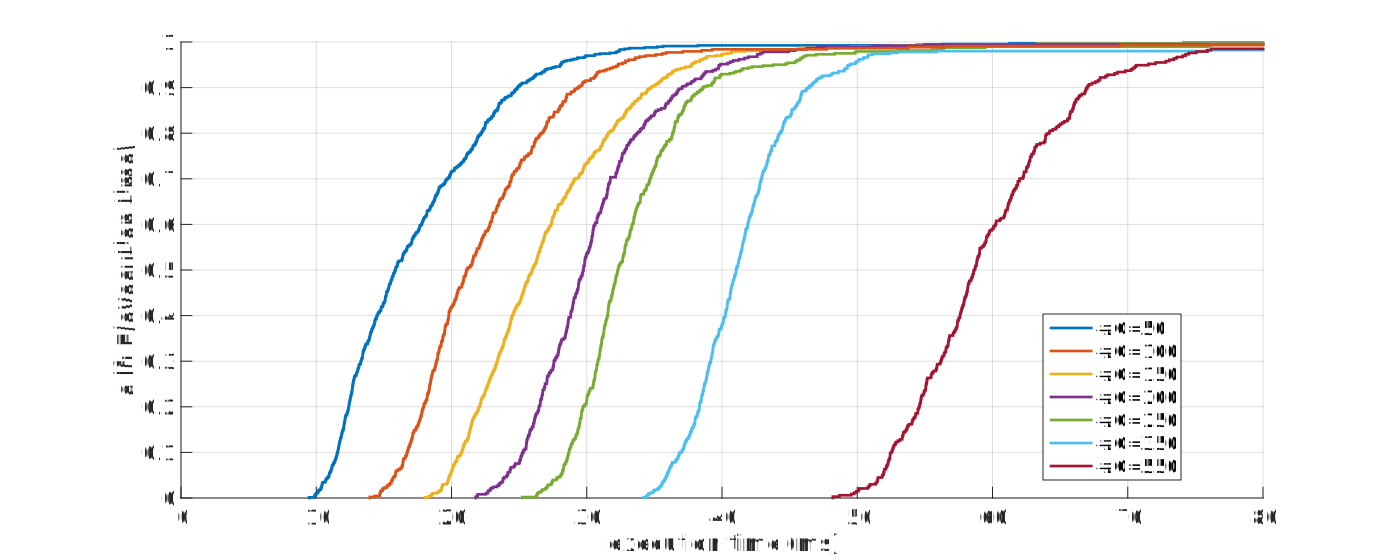
\includegraphics[width=0.9\columnwidth]{figures/time_ecdf_millisec.pdf}
  \caption{Cumulative distribution of profiled execution times for visual odometry running on the Odroid-U3 for varying maximum number of corners from the SVO algorithm.}
  \label{fig:time_ecdf}
\end{figure}



\subsection{Experimental Evaluation}

After profiling the performance of the perception and estimation algorithm and formulating the Robust Adaptive MPC controller for the hexrotor linearized around hover and modelled as an LTI system (Eq.~\ref{eq:plant-cont-model}), we experimentally evaluate the tracking performance and estimated energy consumption based on actual flights around a pre-defined trajectory. 
For comparison, we use a Model Predictive Controller with the same cost function and initial feasible sets as in our Robust MPC formulation. 
The MPC controller is an appropriate baseline against which to measure the benefits of our co-design method, as it is a similar control algorithm that does not leverage co-design and is unaware of the estimator algorithm that gives it a state estimate. 

For the evaluation, we fly in a predefined circular trajectory, repeating the experiment 10 times to gather enough data to conclusively measure the performance of RAMPC for different values of $\alpha$ and MPC with fixed modes of ($\delta,\epsilon$). 
Note that since the controller was a sampled discrete-time controller working with simulated 20Hz camera updates, this realistically restricts us to using modes of estimator operation with delay $\delta$ less than 1/20s, or one sampling period, i.e. modes corresponding to 50, 100, 150 and 200 maximum corners from the FAST detector (see Fig. \ref{fig:svo_error_delay}). 
These modes and their estimated power consumption is in Table \ref{tbl:modes_exp}. 
Note, \#C represents the maximum number of FAST corners requested, $\epsilon$ shows the worst case error bound on the state estimate, $\delta$ is the $90^{th}$ percentile execution time for that mode, and $P$ represents the expected power consumption in that mode as profiled offline. 
This power consumption is the computation power used by a particular mode in excess to the idle power for the Odroid used for profiling, which was 1.5W.

\begin{table}[htb]
\begin{center}
\caption{Estimation modes used in the experiment.}
\label{tbl:modes_exp}
\begin{tabular} {|c|c|c|c|c|}
	\hline
	\textbf{Mode} & \textbf{\#C} & $\pmb{\epsilon}$ & $\pmb{\delta}$ \textbf{(ms)} & $\pmb{P}$\textbf{(W)} \\ \hline
	0 & 50 &  24.88 & 0.028 &  0.778  \\ \hline
 	1 & 100 & 29.82 & 0.0237 &  0.862  \\ \hline
	2 & 150 & 34.66 & 0.0230 & 0.870 \\ \hline
	3 & 200 & 38.01 & 0.0113 & 0.951 \\ \hline
	\end{tabular}	
	\end{center}
\end{table}




\subsection{Experimental Results}

Once the flights are complete, to get a more accurate picture of how the controllers really performed, we use the following function to measure tracking performance at each time step.

\begin{equation}
	J_{true}(t) =  (x(t)-x_{ref}(t))^{T}Q(x(t)-x_{ref}(t)) + u(t)^{T}Ru(t)
\end{equation}

Note that since we have access to the true position and velocities ($x(t)$) of the hexrotor with the VICON system, we can obtain the true tracking cost. Table \ref{tbl:RAMPC_MPC_performance} shows the mean of the above function over the 10 flights for both MPC across all fixed modes and RAMPC with different values of $\alpha$. It also shows the estimated energy consumption based on the time spent in each mode (which can be seen in Table \ref{tbl:RAMPC_ModeTime} for RAMPC). RAMPC shows better tracking performance (lower mean $J_{true}$) than the MPC with either of the 4 fixed modes, showing the improved control performance that can be obtained by dynamically switching between estimation modes in-flight at runtime. 

\begin{figure}[tbh]
	\centering
	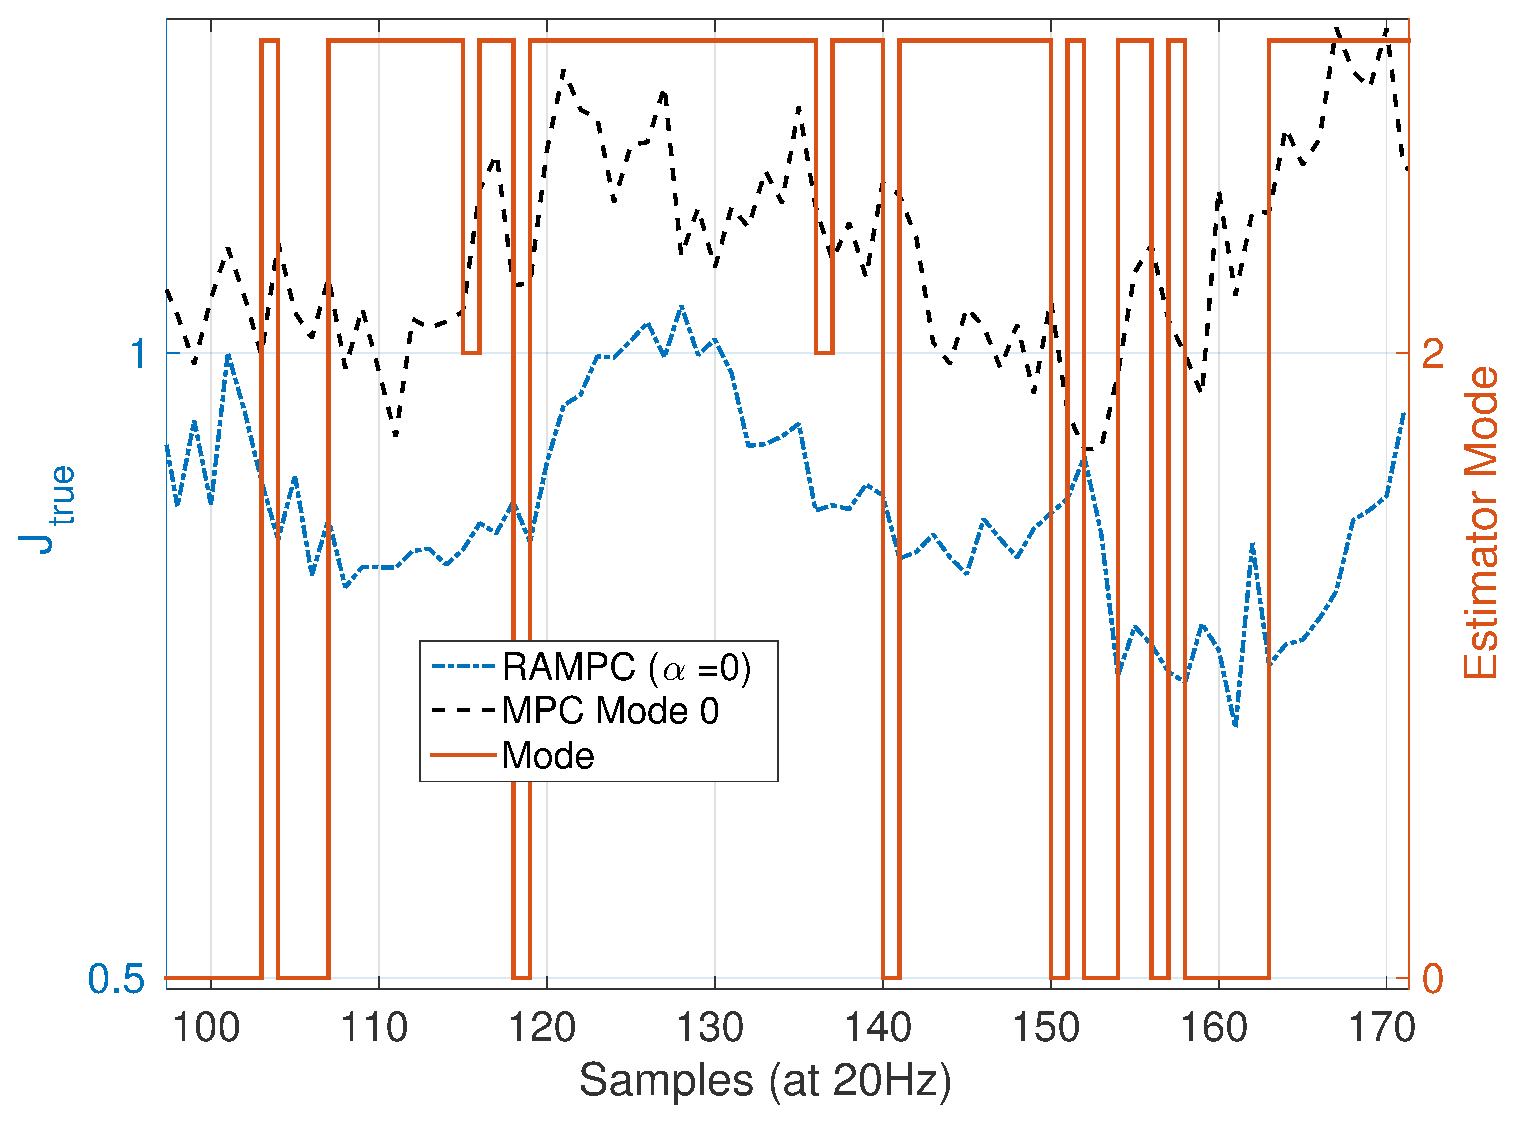
\includegraphics[width=0.49\textwidth]{figures/CostAndModes}
	\caption{Tracking cost at each time step for MPC (fixed mode 0 estimator) and RAMPC with $\alpha=0$. Note how the RAMPC performs better (lower cost) than the MPC and there is dynamic switching of estimator modes at runtime leading to improved performance for the RAMPC.}	
	\label{fig:CostAndModes}
\end{figure}


Figure \ref{fig:CostAndModes} shows how the tracking cost ($J_{true}$) evolves over time for RAMPC (with $\alpha=0$) and MPC (fixed mode 0) for a portion of the hexrotor flight. The estimator modes selected by RAMPC are overlaid in orange. Figure \ref{fig:CostAndModes} demonstrates that RAMPC has uniformly lower tracking cost than MPC, enabled by RAMPC's dynamic switching of estimator modes at runtime. Note that RAMPC exhibits better tracking performance throughout the flight and not just in this portion, and also outperforms MPC at other modes (see Table \ref{tbl:RAMPC_MPC_performance}).

Figure \ref{fig:TrackingVsEnergy} shows that RAMPC provides better tracking performance while using less energy to do so. For any fixed energy budget (a point on the x-axis), RAMPC delivers lower tracking cost (y-axis) than MPC. While MPC's tracking error is relatively constant across modes, RAMPC is able to balance tracking error with energy consumption by varying the $\alpha$ parameter. RAMPC's switching between estimation modes improves not only the control performance but also energy efficiency.


\begin{figure}[tbh]
	\centering
	\includegraphics[width=0.49\textwidth]{figures/TrackingVsEnergy}
<<<<<<< HEAD
	\caption{Tracking cost vs estimated computation energy for executing the perception and estimation algorithm. Note for MPC, different energies are realized only by operating at different fixed modes of the perception and estimation algorithm. Using RAMPC as the controller, the different energies are due to run-time scheduling of different modes based on the optimal value of the cost function \ref{eq:tractableOptim} at each time step based on different values of $\alpha$. It is worth noting that RAMPC with co-design outperforms standard MPC on tracking performance across the entire range of energy consumption.}
=======
	\caption{Tracking cost vs estimated computation energy for executing the perception and estimation algorithm. Note for MPC, different energies are realized only by operating at different fixed modes of the perception and estimation algorithm. Using RAMPC as the controller, the different energies are due to run-time scheduling of different modes based on the optimal value of the cost function of Eq. \ref{eq:tractableOptim} at each time step based on different values of $\alpha$. It is worth noting that RAMPC with co-design outperforms standard MPC on tracking performance across the entire range of energy consumption.}
>>>>>>> 7670c209058446b377ea51df3df0ba33181e588d
	\label{fig:TrackingVsEnergy}
\end{figure}


\begin{table}[htb]
\begin{center}
\caption{Tracking performance and computation energy}
\label{tbl:RAMPC_MPC_performance}
\begin{tabular} {|c|c|c|c|c|}
	\hline
	\textbf{Controller} &\textbf{Est. Mode}/ $\pmb{\alpha}$ & $\pmb{E[J_{true}]}$ & $\pmb{\sigma({J_{true}})}$ & $\pmb{Energy(J)}$ \\ \hline
	MPC & 0/ $-$ & 1.0903 & 0.104 & 43.89\\ \hline
	MPC & 1/ $-$ & 1.0878 & 0.087 & 49.02 \\ \hline
	MPC & 2/ $-$ & 1.0760 & 0.098 & 49.60 \\ \hline
	MPC & 3/ $-$ & 1.0762 & 0.088 & 54.15 \\ \hline
	RAMPC &  $-$/0 & 0.8836 & 0.079 & 49.28 \\ \hline
	RAMPC & $-$/ 0.001 & 1.0029 & 0.093 & 48.90  \\ \hline
	RAMPC & $-$/ 0.01 & 1.0280 & 0.089 & 48.69  \\ \hline
	RAMPC & $-$/ 0.05 &1.0302 & 0.096 & 46.33 \\ \hline
	RAMPC & $-$/ 0.1 &1.0601 & 0.086 & 46.01 \\ \hline
	RAMPC & $-$/ 0.2 & 1.0776 & 0.083 & 44.49 \\ \hline
\end{tabular}	
	\end{center}
\end{table}



Figure \ref{fig:CostAndEnergyVsAlpha} shows the degradation (increased mean $J_{true}$) in tracking performance and reduction in energy consumption as the weight $\alpha$ for the computation power consumption in the cost function is increased. As energy becomes more important, RAMPC smoothly balances tracking cost and energy consumption. Table \ref{tbl:RAMPC_ModeTime} quantifies how RAMPC makes this trade-off, by showing the fraction of time spent in the 4 modes with RAMPC as $\alpha$ changes. While time is split between modes 0 and 3 with $\alpha=0$, more and more time is spent in the low-power (but less accurate) mode 0 as $\alpha$ increases.


\begin{figure}[t]
	\centering
	\includegraphics[width=0.49\textwidth,scale=0.7]{figures/CostAndEnergyVsAlpha}
        \vspace{-20pt}
	\caption{RAMPC tracking cost and estimated computation energy for the perception and estimation algorithm as a function of $\alpha$. }
	\label{fig:CostAndEnergyVsAlpha}
\end{figure}


\begin{table}[htb]
\begin{center}
\caption{Fraction of time spent in different estimator modes as $\alpha$ changes for RAMPC}
\label{tbl:RAMPC_ModeTime}
\begin{tabular} {|c|c|c|c|c|}
	\hline
	$\pmb{\alpha}$ & \textbf{Mode 0} & \textbf{Mode 1} & \textbf{Mode 2} & \textbf{Mode 3} \\ \hline
	0 & 0.461 & 0.009 & 0.020 & 0.510 \\ \hline
 	0.001 &  0.494 & 0.001 & 0.029 & 0.467 \\ \hline
	0.01 & 0.512 & 0.005 & 0.039 & 0.444  \\ \hline
	0.005 &  0.692 & 0.000 & 0.156 & 0.152 \\ \hline
	0.1 & 0.691 & 0.000 & 0.218 & 0.091 \\ \hline
	0.2 & 0.897 & 0.000 & 0.098 & 0.005  \\ \hline
	\end{tabular}	
	\end{center}
\end{table}



\input{discussion}
\section{Conclusion}
\label{conclusion}

In this paper we presented a contract-based methodology for co-design of estimation and control for autonomous systems. 
The basic idea is that the control algorithm requests a time and estimation error $\de$ contract that the perception-and-estimation algorithm realizes. The control algorithm we designed aims to set time varying contracts to maximise a performance function while guaranteeing feasibility constraints and stability under the time varying execution time and estimation error from the estimator. We also illustrate how the contract based perception-and-estimation algorithm is designed offline and used at run-time to best meet the $\de$ contracts set for it. Through a case study on a flying hex-rotor, we showed the applicability of our scheme to real-time closed loop system. The experimental results show the good performance of our scheme and how it outperforms regular Model Predictive Control which does not leverage co-design. A key result showed how our closed loop solution is more energy efficient than MPC while achieving better tracking performance. A focus of ongoing research is to overcome the necessity of the contracts always being met by the estimator in order of us to have strong mathematical guarantees for the control performance. Another focus is on an automated tool chain to profile perception algorithms commonly used in autonomous systems.

\bibliographystyle{abbrv}
\bibliography{rtss2015}  




\end{document}
